\documentclass{book}
\usepackage{xeCJK}
\usepackage{ctexcap}
\usepackage{bm}
\usepackage{amsmath,amssymb,amsfonts}
\usepackage{float}

\begin{document}
\chapter{三相变压器}
现代电力系统都采用三相制,因而三相变压器得到广泛的应用。三相变压器可以由三台 相同的单相变压器组合而成,称为三相变压器组,其结构示意图见图\ref{fig_4.1};也可以将三相铁心做成一体,称为三相心式变压器,其铁心结构示意图见图\ref{fig_4.2}。
\begin{figure}[H]
	\centering
	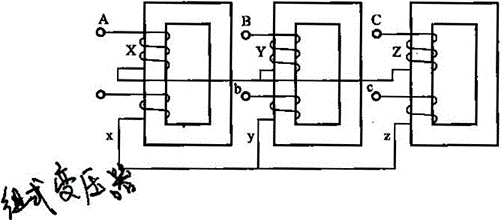
\includegraphics[width=0.80\textwidth]{4-1.png}
	\caption{三相变压器组结构示意图}
	\label{fig_4.1}
\end{figure}
\begin{figure}[H]
	\centering
	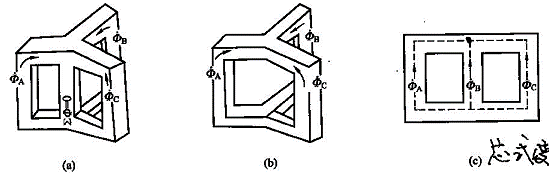
\includegraphics[width=0.80\textwidth]{4-2.png}
	\caption{三相心式变压器铁心结构示意图
		(a)结构一;(b)结构二;(c)结构三}
	\label{fig_4.2}
\end{figure}

三相变压器,在对称运行时,取其一相分析,能量转换过程和一、二次侧电压、电流关系,都与单相变压器相同。因此,有关三相变压器运行原理、分析计算方法等方面的问题不 再叙述。至于三相变压器在不对称运行时的分析计算方法,留待第五节中做详细的讨论。

本章将重点介绍三相变压器在磁路系统和电路系统中不同于单相变压器的特点,并讨论 三相变压器的绕组连接方式和铁心结构对变压器空载电动势波形的影响。

\section{三相变压器的磁路系统}

\subsection{三相变压器组}
将三台相同的单相变压器的一、二次侧,分别按一定方式进行三相连接,则可组成三相 变压器组,其结构示意图如图\ref{fig_4.1}所示。从电路上看,三相是互相连接的,但在磁路上三相是彼此独立的,即三相之间只有电的联系而无磁的联系。与三相心式变压器相比,三相变压器组有下列优点。

(1)在变电所中,为防止因变压器故障损坏或定期检修而造成停电,往往需存放一台备 用的变压器。由于三相变压器组是由三台独立的单相变压器组合而成的,所以只需要备用一 台单相变压器.与同容量的三相心式变压器相比,其备用容量降为三分之一。

(2)对于巨型变压器,选用三相变压器组时,其每台单相变压器的容量只为总容量的三分之一,故体积小、重量轻、便于运输。
\subsection{三相心式变压器}

如将图\ref{fig_4.1}中的三台单相变压器不套绕组的铁心柱合在一起,则得到图\ref{fig_4.2}所示的铁心结构。这时,在中央公共铁心柱中流过的磁通应为三相磁通的相量和。当外加三相电压对称时,三相磁通最大值相等,相位互差120°,所以中央公共铁心中的磁通为
\begin{equation}
\phi ={{\phi }_{A}}+{{\phi }_{B}}+{{\phi }_{C}}=0
\label{3-57}
\end{equation}
这样可以省去中央的铁心柱,铁心便演变为图\ref{fig_4.2}(b) 所示的形状。这时三相磁通的流通情况,类似于星形元中性线三相对称电路中的电流的流通情况,即三相互为回路。

为了节省材料和制造工艺上的方便,再将三相的铁心柱安排在一个平面内,于是得到图\ref{fig_4.2}(c)所示的铁心形状。这种铁心结构,中间一相的磁阻较小,所以其励磁电流也比另外两相小。由于变压器的励磁电流相对于额定电流是很小的,所以这种不对称对变压器的运行性能并无明显的影响。

与同容量的三相变压器组相比,三相心式变压器的主要优点是节省材料、降低成本、缩 小体积、方便管理,因此一般中小容量的电力变压器都采用三相心式变压器。只有大功率的巨型变压器,为了运输上的方便和减少备用投资,才采用三相变压器组。


\section{三相变压器的电路系统}
\subsection{三相绕组的连接方法}
在三相变压器中,通常用大写字母A、B、C表示一次绕组的首端,用X、Y、Z表示一次绕组的末端。用小写字母a、b、c表示低压绕组的首端,用x、y、z表示二次绕组的末端。
从理论上讲,三相变压器的一、二次绕组都可连接成星形成三角形。所谓星形连接,就是将三相绕组的末端连在一起,作为中性点,而将三个首端引出如图 4 3(a)所示。当无中性线引出时用符号Y(y)表示,当有中性线引出时用符号YN(yn)表示。所谓三角形连接,就是将一相绕组的末端与另一相绕组的首端相连,顺次连成一个闭合回路,图 4 3(b)和(c)所示为两种连接顺序不同的三角形连接。三角形连接的表示符号为D(d)。

\begin{figure}[H]
	\centering
	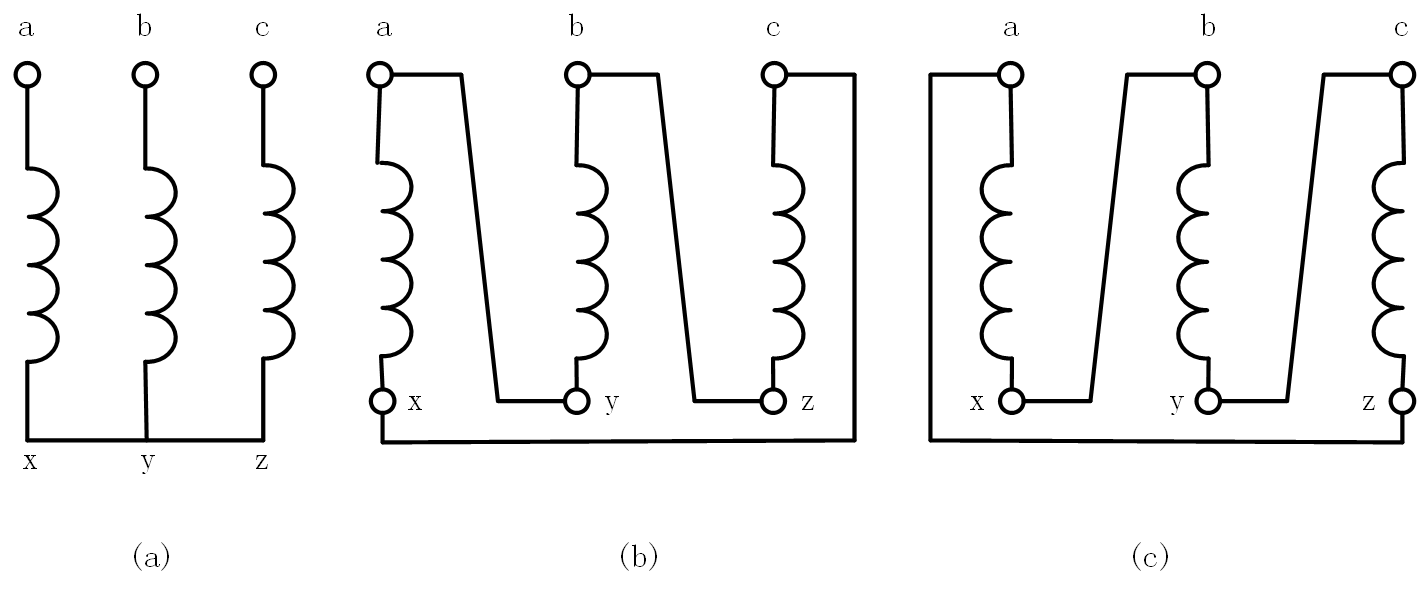
\includegraphics[width=0.80\textwidth]{4-3.png}
	\caption{三相绕组的连接法
		(a)结构一;(b)结构二;(c)结构三}
	\label{fig_4.3}
\end{figure}

我国生产的三相电力变压器主要采用Yyn、Yd和YNd连接方式。

对于三相变压器,变比k是指一、二次侧每相的匝数比。与単相変圧器一样,三相变压器相电压之比也近似地等于变比k。但在使用变压器变换三相电压时,人们更为关心的是三相变压器的线电压之比,称为三相变压器的变压比。显然,三相变压器的变压比除与变比k有关外,还与一、二次绕组的连接方式有关。当三相变压器绕组连接为Yy时,其变压比近似等于变比k;当绕组连接为Yd时,其变压比近似等于$\sqrt{3}k$。

\subsection{绕组间的同极性端}

在使用三相变压器时,不但要知道一、二次侧线电压的数值关系(即变压比),有时还要知道它们的相位关系。为了分析这方面的问题,必须先明确有关同极性端的概念。

对于直流电源,其两极的极性是不变的。两个电池的正极为同极性端,它们的负极也是同极性端。而对变压器的绕组,其两个端头的正、负极性是不断变化的,没有固定的极性。但对连接同一主磁通的两个绕组来说,当一个绕组的某一端头为正极性时,在另一个绕组上也必定有一个端头为正极性。这种同时为正、同时为负的两个端头称为两绕组的同极性端,用符号“$\centerdot $”表示。确定绕组间的同极性端时,必须注意绕组的绕向。先在图中给出磁通$\phi $的正方向,然后按右手螺旋关系画出两绕组中感应电动势${{e}_{1}}$和${{e}_{2}}$的正方向。根据${{e}_{1}}$和${{e}_{2}}$同相位的关系,可立即判定两绕组的同极性端,如图\ref{fig_4.4}所示。
\begin{figure}[H]
	\centering
	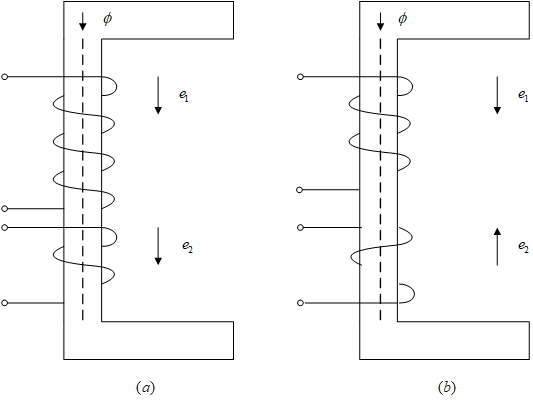
\includegraphics[width=0.80\textwidth]{4-4g.png}
	\caption{绕组间的同极性端
		(a)同向;(b)异向
	}
	\label{fig_4.4}
\end{figure}

\subsection{三相变压器的连接组}
在三相变压器的铭牌上标有连接组,例如 Yd11。它既能反映一、二次绕组各自的连接 方式,又能反映一、二次绕组对应线电压的相位关系。为什么组号11能反映电压间的相位 关系呢?这是因为采用了时针表示法,将一、二次绕组的对应线电压画在同一相量图中,用相量${{U}_{ab}}$ 表示时针,它所指示的时钟数就定为连接组的组号。例如在图图\ref{fig_4.5}中,
\begin{figure}[H]
	\centering
	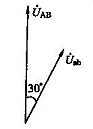
\includegraphics[width=0.80\textwidth]{4-5.png}
	\caption{时针表示法}
	\label{fig_4.5}
\end{figure}
${{U}_{ab}}$ 滞后于${{U}_{ab}}$30°,则定其连接组号为1。下面对Yy连接和Yd连接的连接组号分别进行讨论。为便于分析,近似地用电动势代表其对应的电压。

关于各电动势的正方向,进行如下规定:Y连接时,各相电动势的正方向一律从各相首端指向中性点;线电动势的正方向从电动势下标中第一个字母指向第二个字母,例如${{\dot{E}}_{AB}}$ 的正方向应从A指向B。D连接时,线电动势等于对应的相电动势,各电动势的正方向都应从其下标中第一个字母指向第二个字母,例如${{\dot{E}}_{bc}}$的正方向应从b指向c。

\subsubsection{Yy连接}

在图、中,由于未画出铁心,看不出一、二次绕组的绕向,这时必须用符号“$\centerdot $”标明同相两绕组的同极性端,否则就无法判断二者电动势的相位关系。
\begin{figure}[H]
	\centering
	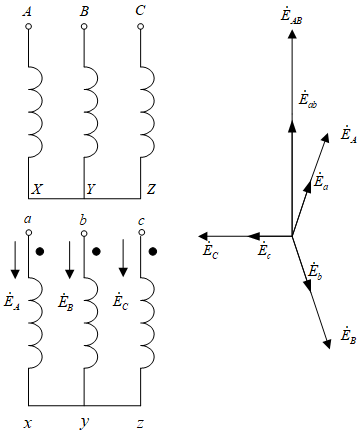
\includegraphics[width=0.80\textwidth]{4-6g.png}
	\caption{Yy0连接组}
	\label{fig_4.6}
\end{figure}
图\ref{fig_4.6}中,根据同极性端和电动势的正方向可以判定一、二次绕组各对应相电动势同 相位,由相量图可知,它们的对应线电动势${{\dot{E}}_{AB}}={{\dot{E}}_{A}}-{{\dot{E}}_{B}}$ 和${{\dot{E}}_{ab}}={{\dot{E}}_{a}}-{{\dot{E}}_{b}}$也是同相位的。因此,称为Yy0连接组。
如果保持接线和一次绕组各端头的标志不变,而将二次绕组的端头b改为a,c改为b,a改为c,这时二次绕组相序仍与一次绕组一致,只是电动势${{\dot{E}}_{a}}$不再与${{\dot{E}}_{A}}$同相位,而是与${{\dot{E}}_{B}}$同相位,即比改变前滞后了120°。同理,${{\dot{E}}_{b}}$、${{\dot{E}}_{c}}$以及线电动势${{\dot{E}}_{ab}}$都比改变前滞后了120°,用时钟表示法,其连接组号应增加为4,所以这时的变压器为Yy4 连接组。
如保持图\ref{fig_4.6}中接线和一次绕组各端头的标志不变,而将二次绕组中的c改为a,a改 为b,b改为c,其相序仍与一次绕组一致,只是${{\dot{E}}_{a}}$与高压绕组的${{\dot{E}}_{C}}$同相位,比改变前滞后了240°,显然,线电动势${{\dot{E}}_{ab}}$也比改变前滞后了240°,其连接组号应增加8,这时的变压器为Yy8连接组。
\begin{figure}[H]
	\centering
	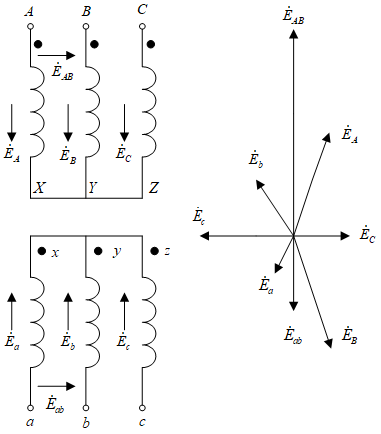
\includegraphics[width=0.80\textwidth]{4-7g.png}
	\caption{Yy6连接组}
	\label{fig_4.7}
\end{figure}
在图\ref{fig_4.7}中,每相一、二次绕组的首端取在非同极性端上,一、二次绕组各对应相电动势相位相反。显然,对应线电动势${{\dot{E}}_{ab}}$和${{\dot{E}}_{AB}}$的相位也相反,按时钟表示法,这时的连接组号为6,即变压器为Yy6 连接组。
保持接线不变,用上述改变二次绕组首端标志的方法,可以得到Yy10和Yy2连接组。

\subsubsection{Yd连接}

在图\ref{fig:4.8}中,二次绕组的线电动势${{\dot{E}}_{ab}}$就等于中间相(即ab相)的相电动势,而后者与一次绕组的相电动势${{\dot{E}}_{B}}$反相位。由相量图可知,${{\dot{E}}_{ab}}$滞后于${{\dot{E}}_{AB}}$330°,所以它是 Yd11连接组。
\begin{figure}  %两个图片并排放
	\begin{minipage}[H]{0.45\linewidth}  
		\centering  
		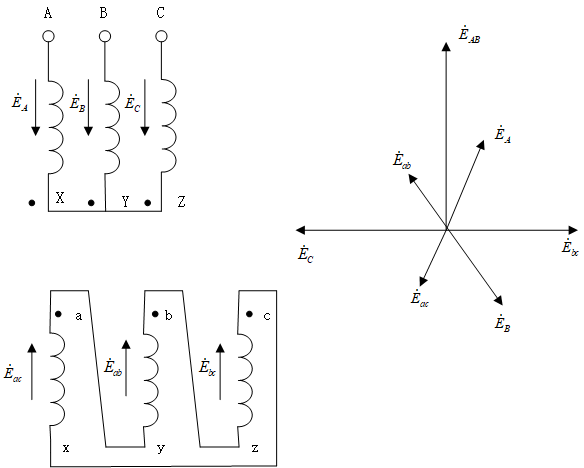
\includegraphics[width=2.2in]{4-8g.png}  
		\caption{Yd11连接组}  
		\label{fig:4.8}  
	\end{minipage}
	\begin{minipage}[H]{0.45\linewidth}  
		\centering  
		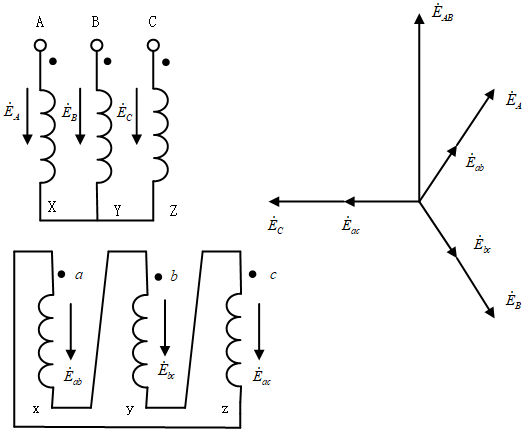
\includegraphics[width=2.2in]{4-9g.png}  
		\caption{Yd1连接组}  
		\label{fig:4.9}  
	\end{minipage}  
\end{figure}

如果保持接线和一次绕组各端头的标志不变,而将二次绕组中的b改为a,c改为b,a改为c,则${{\dot{E}}_{ab}}$与高压绕组的${{\dot{E}}_{c}}$反相位,可得Yd3连接组。如把c改为a,a改为b,b改为c,则${{\dot{E}}_{ab}}$与${{\dot{E}}_{A}}$反相位,可得Yd7连接组。

在图\ref{fig:4.9}中,二次绕组的线电动势${{\dot{E}}_{ab}}$就等于ab相的相电动势,而后者与一次绕组的相电动势${{\dot{E}}_{A}}$同相位。由相量图可知,${{\dot{E}}_{ab}}$滞后于${{\dot{E}}_{ab}}$ 30°,所以它是Yd1连接组。保持接线不变,用上述改变低压绕组首端标志的方法,可以得到 Yd5 和 Yd9 连接组。
综上所述,Yy连接的连接组号共有2、4、6、8、10、12六种,Yd连接的连接组号共有1、3、5、7、9、11六种。而在实际中,为了使用上的方便,并不采用这么多种连接组,我国国家标准规定只生产五种标准连接组,即Yyn0、Yd11、YNd11、YNy0、YyO。其最常用的为前三种。

\section{三相变压器的空载电动势波形}

由第二章对空载电流波形的分析中得到,当磁路饱和时,为了保证主磁通$\Phi$和主磁电动势${{e}_{1}}$、${{e}_{2}}$为正弦波,空载电流${{i}_{0}}$必须为尖顶波。尖顶波按傅氏级数可分解为基波和各奇次谐波,高次谐波中三次谐波是构成尖顶波的主要成分(见图\ref{fig:4.10})。
\begin{figure}  
	\begin{minipage}[H]{0.45\linewidth}  
		\centering  
		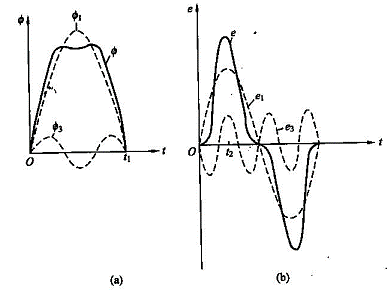
\includegraphics[width=2.2in]{4-10.png}  
		\caption{尖顶波的基波和三次谐波}  
		\label{fig:4.10}  
	\end{minipage}
	\begin{minipage}[H]{0.45\linewidth}  
		\centering  
		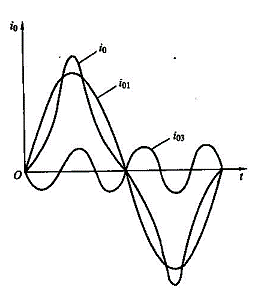
\includegraphics[width=2.2in]{4-11.png}  
		\caption{非正弦的磁通和电动势
			(a)磁通曲线图;(b)电动势曲线图}  
		\label{fig:4.11}  
	\end{minipage}  
\end{figure}
在単相変圧器中,基波${{i}_{01}}$和二次谐披${{i}_{03}}$都可顺利通过一次侧,从而得到尖顶波的空载电流${{i}_{0}}$。而在三相变压器中,A、B、C 三相空载电流的基波互差120°,三次谐波互差3×120°=360°,即
\begin{align}
& {{i}_{03A}}=\sqrt{2}{{I}_{03}}\sin 3\omega t \\ 
& {{i}_{03B}}=\sqrt{2}{{I}_{03}}\sin 3\left( \omega t-120{}^\circ  \right)=\sqrt{2}{{I}_{03}}\sin 3\omega t \\ 
& {{i}_{03C}}=\sqrt{2}{{I}_{03}}\sin 3\left( \omega t-240{}^\circ  \right)=\sqrt{2}{{I}_{03}}\sin 3\omega t
\label{4-2}
\end{align}
由于三相空载电流的三次谐波同相位,它能否顺利流通与三相绕组的连接方式有关,如果一次侧为${{Y}_{0}}$连接,三次谐波电流可以通过中性线流通,故${{i}_{0}}$为尖顶波,因而不会引起磁通和电动势的非正弦畸变。对于一次侧的其他连接方式,则要分类进行讨论。

\subsection{Yy连接}
下面的分析也适用于Y连接,因为Yyn 连接在空载时也相当于Yy 连接。

由于一次侧为星形无中性线连接,所以空载电流${{i}_{0}}$的三次谐波无法流通,结果使${{i}_{0}}$接近于正弦波。当磁路饱和时,主磁通$\phi $近于平顶波,与尖顶波类似,平顶波的主要成分也是基波和三次谐波,如图\ref{fig:4.11}(a)所示。而三次谐波磁通${{\phi }_{3}}$的流通情况则与变压器磁路的结构形式有关,下面分两种情况讨论。


\subsubsection{三相变压器组}
虽然三相的三次谐波磁通同相位,但由于三相变压器的磁路是三相彼此独立的,三次谐波磁通${{\phi }_{3}}$可以顺利通过铁心。另外,三次谐波的频率${{f}_{3}}$为基波的三倍,所以${{\phi }_{3}}$将在一、二次绕组中产生较大的三次谐波电动势${{e}_{3}}$,其幅值可达基波电动势${{e}_{1}}$幅值的45\% \textasciitilde60\%。在图\ref{fig:4.11}(a)中,对应${{t}_{1}}$时刻,${{\phi }_{1}}$和${{\phi }_{3}}$都有负的最大变化率,根据公式$e=-N\frac{\text{d}\phi }{\text{d}t}$,这时的${{e}_{1}}$和${{e}_{3}}$都应有正的最大值,相当于图\ref{fig:4.11}(b)中的${{t}_{2}}$时刻,${{e}_{1}}$和${{e}_{3}}$(请确认)叠加起来,就得到一个尖顶波的相电动势$e$。电动势$e$的幅值比设计值高很多,可能造成绕组绝缘的损坏。因此,三相变压器组不能采用Yy和。。。连接。

还应指出,三次谐波电动势只存在于每相绕组中,而在线电动势中不含有三次谐波分量。因为三相的三次谐波电动势同相位,即${{\dot{E}}_{3A}}={{\dot{E}}_{3B}}={{\dot{E}}_{3C}}$,而电动势${{\dot{E}}_{3AB}}={{\dot{E}}_{3A}}={{\dot{E}}_{3B}}=0$。

\subsubsection{三相心式变压器}

其三相磁路相连,如同星形无中性线的电路一样。对于三相同相位的三次谐波磁通,它 是无法在这样的磁路内流通的。在这种憧况下,三次谐波磁通被迫穿过变压器油流经油箱壁闭合。由于这时磁路的磁阻很大,所以三次谐波磁通及其感生的三次谐波电动势都变得很 小,一、二次侧的空载电动势基本上为正弦波。因此,三相心式变压器可采用Yy和Yyn连接。通过油箱壁的三次谐波磁通以3倍电网频率交变,从而在油箱壁中产生一定的涡流损耗。为保证变压器有较高的运行效率,较大容量的三相心式变压器也不采用Yy连接。

\subsection{Yd连接}
\subsubsection{作升压变压器用时}
一次侧绕组为D连接,由于无中性线,电源也无法提供具有三次谐波的空载电流,即${{i}_{0}}$近于正弦波。当磁路饱和时,主磁通近于平顶波,也就是说在铁心中将出现三次谐波磁通${{\phi }_{3}}$。${{\phi }_{3}}$在一、二次侧绕组内产生三次谐波电动势${{e}_{3}}$。因为三相绕组中的${{e}_{3}}$同相位,它们在一次绕组($\Delta $)电路内将产生环流${{\dot{I}}_{3}}=\frac{3{{{\dot{E}}}_{3}}}{3{{{\dot{Z}}}_{3}}}$,如图\ref{fig_4.12}所示。

由于频率高,所以在阻抗${{Z}_{3}}$中感抗远大于电阻,可近似地认为${{i}_{3}}$在相位上滞后${{e}_{3}}90{}^\circ $,即与${{\phi }_{3}}$近于反相位。由于${{i}_{3}}$的去磁作用,使${{i}_{3}}$和${{e}_{3}}$都变得很小,结果使铁心的总磁通和绕组中的总磁动势都近似为正弦波。也可以这样认为:电源向每相供给的基波电流加上绕组内感生的三次谐波电流,共同形成了一个尖顶波的空载电流,从而保证了磁通和电动势基本上为正弦波。

\begin{figure}[H]
	\centering
	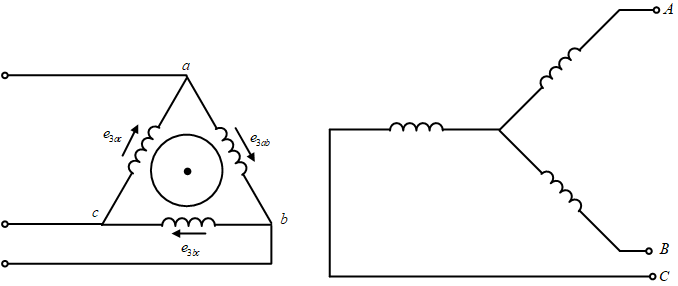
\includegraphics[width=0.80\textwidth]{4-12g.png}
	\caption{三角形电路内的三次谐波环流}
	\label{fig_4.12}
\end{figure}

\subsubsection{作降压变压器用时}
一次绕组为Y连接,空载电流中也没有三次谐波分量,即${{i}_{0}}$近于正弦波。与上面分析一样,这时将出现三次谐波磁通${{\phi }_{3}}$,只是它不能在一次绕组中感生三次谐波电流,而在二次侧 D连接绕组内感生三次谐波环波${{i}_{3}}$。${{i}_{3}}$削弱${{\phi }_{3}}$,从而使总磁通和绕组电动势近似为正弦波,也可认为:一次侧空载电流所产生的基波电动势与二次侧中${{i}_{3}}$所产生的三次谐披磁动势,在铁心中合成一个尖顶波磁动势,从而保证了主磁通和绕组电动势基本为正弦波。

综上所述,三相变压器一、二次绕组只要有一端为D连接,即可保证空载电动势基本上为正弦波。因此,三相变压器组合较大容量的心式变压器都采用 Yd11连接组,而Yy和Yyn连接主要用于功率不大的三相心式变压器。当大功率电力变压器需要一、二次侧都接成 Y 时,在铁心上加装一个接成 D 的小容量的第三绕组,它不向外输出功率,仅产生三次谐波环流,以改善相电动势的波形。

\section{变压器的并联运行}
\subsection{并联运行}
在现代发电厂和变电所中,常采用多台变压器并联运行的方式供电。所谓并联运行,就是将各台变压器的一次测并联在一起,通过公共母线接于同一电源,二次侧并联在一起,通过公共母线向共同的负载供电(见图\ref{fig_4.13})。
与单台变压器供电相比,并联运行有以下主要优点。

\begin{figure}[H]
	\centering
	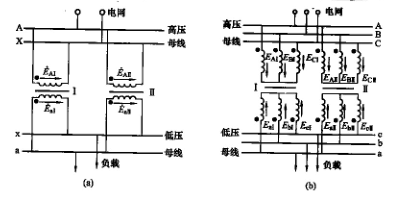
\includegraphics[width=0.80\textwidth]{4-13.png}
	\caption{变压器并联运行接线示意图
		(a)单相变压器;(b)三相变压器}
	\label{fig_4.13}
\end{figure}

(1)数台变压器并联运行,当某台变压器发生故障或需要检修时,可将它从电网上切除,而其余的变压器仍可继续供电,从而保证重要负载不断电。因此,并联运行可提高供电的可靠性。

(2)变压器二次侧负载的大小是随时间不断变化的,而变压器在轻载时效率较低。并联运行时,可根据负载的需要决定投入的变压器台数,以使其工作在效率较高的状态,这样就提高了运行的经济性。

(3)由于并联运行时单台变压器的容量较小,所以可减小变电所的备用容量。另外,可 随着用电量的增加,分期地并入新的变压器,以减少初期投资。

应该指出,在每个变电所中并联变压器的台数不宜过多,否则将使设备投资增大,运行管理复杂。

变压器并联运行的理想情况如下:

(1)空载时,并联的各台变压器绕组间无环流。因空载环流将引起附加铜损耗,严重时可能烧毁绕组绝缘。

(2)负载时,输出的电流(或功率)应该按各台变压器的额定容量成正比例地分配。换句话说,就是应使各台变压器的负载系数$\beta $相等。当一台变压器满载时,其余各台变压器也恰好满载,这样就可以保证各台变压器的容量都能得到充分的利用。

(3)负载时,各台变压器的输出电流同相位。这样在各台输出电流一定时,整个并联组可以得到最大的输出电流,即整个并联组有最大的输出容量。

\subsection{理想并联运行的条件}

为了达到上述并联运行的理想情况,必须满足下列条件。

(1)	各台变压器的连接组号相同;

(2)	各台变压器一、二次侧额定电压分别相等,简单地说就是各台变压器的变比相等;

(3)	各台变压器短路阻抗的标幺值$\left| {{Z}_{k}} \right|*$ 相等,即各台变压器的短路电压${{u}_{k}}$相等;

(4)	各台变压器短路阻抗的抗组比$\frac{{{x}_{k}}}{{{r}_{k}}}$ 相等。

不满足第一个条件时,将在变压器绕组中产生很大的空载环流。例如Yy0和Yd11并联时,二次侧对应线电动势在相位上相差30°,在两台变压器二次侧形成的回路中出现电压$\Delta {{\dot{E}}_{2}}$,其大小根据图\ref{fig:4.14}的相量图可求出
\begin{equation}
\Delta {{E}_{2}}=2{{E}_{2}}\sin 15{}^\circ =0.518{{E}_{2}}
\label{4-3}
\end{equation}

\begin{figure}  
	\begin{minipage}[H]{0.45\linewidth}  
		\centering  
		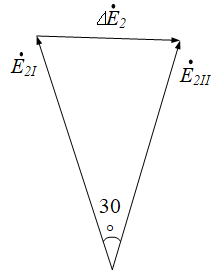
\includegraphics[width=2.2in]{4-14g.png}  
		\caption{尖顶波的基波和三次谐波}  
		\label{fig:4.14}  
	\end{minipage}
	\begin{minipage}[H]{0.45\linewidth}  
		\centering  
		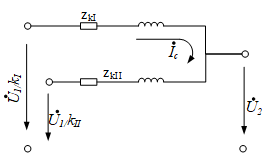
\includegraphics[width=2.2in]{4-15g.png}  
		\caption{非正弦的磁通和电动势
			(a)磁通曲线图;(b)电动势曲线图}  
		\label{fig:4.15}  
	\end{minipage}  
\end{figure}

由于变压器绕组本身的漏阻抗很小,这样大的电动势差将在二次侧形成的回路内产生很大的环流。根据磁动势平衡关系,在两变压器一次侧间也将产生很大的空载环流。因此,连接组相同这一条件必须严格遵守。

不满足第二条件时,即当变压器的变比不相等时,将使各台变压器二次侧的感应电动势出现差值,并在一、二次侧中产生空载环流。图\ref{fig:4.15}所示为变比不等的两台变压器并联运行的简化等效电路。一次侧各量都归算到二次侧,所以短路阻抗${{Z}_{k}}={{Z}_{1}}/{{k}^{2}}+{{Z}_{3}}$。设${{k}_{\text{I}}}<{{k}_{\text{II}}}$,则$\frac{{{U}_{1}}}{{{k}_{\text{I}}}}>\frac{{{U}_{1}}}{{{k}_{\text{II}}}}$,二次侧的空载环流为
\begin{equation}
{{\dot{I}}_{c}}=\frac{\frac{{{U}_{1}}}{{{k}_{\text{I}}}}-\frac{{{U}_{1}}}{{{k}_{\text{II}}}}}{{{Z}_{k\text{I}}}+{{Z}_{k\text{II}}}}
\label{4-4}
\end{equation}

第一台变压器一次侧的环流为$\frac{{{{\dot{I}}}_{c}}}{{{k}_{\text{I}}}}$,第二台变压器一次侧的环流为$-\frac{{{{\dot{I}}}_{c}}}{{{k}_{\text{II}}}}$。在实际中,变比有少许差异,仍允许并联运行。通常规定各台变压器变比间的差值$\Delta k=\frac{\left| {{k}_{\text{I}}}-{{k}_{\text{II}}} \right|}{{{k}_{\text{I}}}{{k}_{\text{II}}}}$ 不超过0.5\%。这时的空载环流一般小于额定电流的5\%。

\begin{figure}[H]
	\centering
	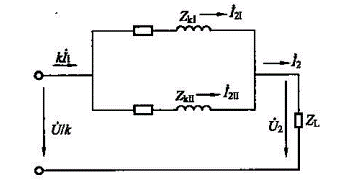
\includegraphics[width=0.80\textwidth]{4-16.png}
	\caption{并联运行归算到二次侧的等效电路}
	\label{fig_4.16}
\end{figure}

下面来分析后两个条件对并联变压器负载运行的影响。图\ref{fig_4.16}所示为并联运行归算到二次侧的等效电路,并假定两台变压器已符合前两个条件。为便于分析,图中的输出电流${{\dot{I}}_{2}}$ 和二次侧电压${{\dot{U}}_{2}}$的正方向,都与图\ref{fig:4.8}中规定的相反。此时${{\dot{I}}_{2}}$与和${{\dot{I}}_{1}}$、${{\dot{U}}_{2}}$和${{\dot{U}}_{1}}$在相位上不再是近于反相位,而是接近于同相位。
由图\ref{fig_4.16}可知
\begin{equation}
{{\dot{I}}_{2\text{I}}}{{Z}_{k\text{I}}}={{\dot{I}}_{2\text{II}}}{{Z}_{k\text{II}}}
\label{4-5}
\end{equation}

由于${{Z}_{k\text{I}}}=\left| {{Z}_{k\text{I}}} \right|\angle {{\varphi }_{k\text{I}}}$,${{Z}_{k\text{II}}}=\left| {{Z}_{k\text{II}}} \right|\angle {{\varphi }_{k\text{II}}}$,所以
\begin{equation}
\frac{{{{\dot{I}}}_{2\text{I}}}}{{{{\dot{I}}}_{2\text{II}}}}=\frac{\left| {{Z}_{k\text{II}}} \right|\angle {{\varphi }_{k\text{II}}}}{\left| {{Z}_{k\text{I}}} \right|\angle {{\varphi }_{k\text{I}}}}=\frac{\left| {{Z}_{k\text{II}}} \right|}{\left| {{Z}_{k\text{I}}} \right|}\angle {{\varphi }_{k\text{II}}}-{{\varphi }_{k\text{I}}}
\label{4-6}
\end{equation}

式(\ref{4-6})中${{\varphi }_{k\text{I}}}$和${{\varphi }_{k\text{II}}}$为两台变压器短路阻抗的阻抗角,其大小为
\begin{align}
& {{\varphi }_{k\text{I}}}=\arctan \frac{{{x}_{k\text{I}}}}{{{r}_{k\text{I}}}} \\ 
& {{\varphi }_{k\text{II}}}=\arctan \frac{{{x}_{k\text{II}}}}{{{r}_{k\text{II}}}}
\end{align}

可见,当两台变压器短路阻抗的抗阻比相等时${{\varphi }_{k\text{II}}}-{{\varphi }_{k\text{I}}}=0$,即两输出电流${{\dot{I}}_{2\text{I}}}$和${{\dot{I}}_{2\text{II}}}$同相位,从而使总输出${{\dot{I}}_{2}}$为最大。在实际中,要使各台变压器的$\frac{{{x}_{k}}}{{{r}_{k}}}$值也相近。通常规定并联变压器的最大容量与最小容量之比不超过3,这样就可保证各台变压器的输出电流间不会有太大的相位差。而当两电流相位差小于20°时,它们的相量和与算术和相差很少,因此,在后面的分析中可近似地认为各并联变压器的输出电流相位相同。因为两台变压器的二次侧额定电压${{U}_{2N}}$ 相同,所以将式(\ref{4-6})端乘以$\frac{1/{{I}_{2N\text{I}}}}{1/{{I}_{2N\text{II}}}}$,右端乘以$\frac{{{I}_{2N\text{II}}}/{{U}_{2N}}}{{{I}_{2N\text{I}}}/{{U}_{2N}}}$,等式仍成立,只是式中各量都化成了他们的标幺值,即
\begin{equation}
\frac{\dot{I}_{2\text{I}}^{*}}{\dot{I}_{2\text{II}}^{*}}=\frac{\left| Z_{k\text{II}}^{{}} \right|*}{\left| Z_{k\text{I}}^{{}} \right|*}\angle {{\varphi }_{k\text{II}}}-{{\varphi }_{k\text{I}}}
\label{4-8}
\end{equation}


可见,当两台变压器短路阻抗标幺值相等时,它们输出电流的标幺值也相等,即两台变 压器的输出电流与它们的额定电流成正比。在实际中并不要求它们的$\left| Z_{k}^{{}} \right|*$绝对相等,通常 规定并联变压器的短路阻抗标幺值相差不超过其平均值的10\%。



\subsection{变压器并联运行时的负载分配}

并联运行的各台变压器一般都保证它们的连接组相同,变比基本相等,但由于规格或容 量的不同,它们的短路阻抗标幺值$\left| Z_{k}^{{}} \right|*$常常有一定的差别。由式(\ref{4-8})知,两台变压器的$\left| Z_{k}^{{}} \right|*$不等时,它们的输出电流标幺值也将不相等。至于输出电流的相位差${{\varphi }_{_{k\text{II}}}}={{\varphi }_{_{k\text{I}}}}$,在并联变压器容量比小于3的条件下;可认为它们的$\frac{{{x}_{k}}}{{{r}_{k}}}$ 基本相等,即${{\varphi }_{_{k\text{II}}}}\approx {{\varphi }_{_{k\text{I}}}}$,于是式(\ref{4-8})可简化为
\begin{equation}
\frac{\dot{I}_{2\text{I}}^{*}}{\dot{I}_{2\text{II}}^{*}}=\frac{\left| {{Z}_{k\text{II}}} \right|*}{\left| {{Z}_{k\text{I}}} \right|*}
\label{4-9}
\end{equation}

因为输出电流的标幺值$I_{2}^{*}$ 就是变压器的负载系数$\beta $,而短路阻抗标幺值$\left| {{Z}_{k}} \right|*$等于变压器的短路电压${{u}_{k}}$,所以(\ref{4-9})也可以写成
\begin{equation}
\frac{{{\beta }_{\text{I}}}}{{{\beta }_{\text{II}}}}=\frac{{{u}_{\text{kI}}}}{{{u}_{\text{kII}}}}
\label{4-10}
\end{equation}

并联变压器负载分配的计算主要有以下两种类型。

(1)	已知各并联变压器的容量、短路电压以及并联组输出的总功率(或电流),求每台变压器的输出功率(或电流)。

如已知两台变压器的额定容量分别为${{S}_{\text{NI}}}$和${{S}_{\text{NII}}}$,短路电压分别为${{u}_{\text{kI}}}$和${{u}_{\text{kII}}}$,总的负载功率为S。为求两台变压器的输出功率${{S}_{\text{I}}}$ 和${{S}_{\text{II}}}$,应列如下方程组,即
\begin{align}
& \frac{{{\beta }_{\text{I}}}}{{{\beta }_{\text{II}}}}=\frac{{{u}_{\text{kII}}}}{{{u}_{\text{kI}}}} \\ 
& S={{S}_{\text{I}}}+{{S}_{\text{II}}}={{\beta }_{\text{I}}}{{S}_{\text{NI}}}+{{\beta }_{\text{II}}}{{S}_{\text{NII}}}
\label{4-11}
\end{align}

解出两变压器的负载系数${{\beta }_{\text{I}}}$和${{\beta }_{\text{II}}}$后,再分别乘以各自的额定容量,可求得两台变压器的输出功率${{S}_{\text{I}}}$ 和${{S}_{\text{II}}}$。

(2)已知各并联变压器的额定容量分别为${{S}_{\text{NI}}}$和${{S}_{\text{NII}}}$,短路电压分别为${{u}_{\text{kI}}}$和${{u}_{\text{kII}}}$。为求并联组的最大输出功率,应设${{u}_{\text{k}}}$值较小的一台的负载系数为1,然后根据式(\ref{4-10})求出另一台的负载系数。用两台的负载系数分别乘以各自额定容量再相加,即得并联组的最大输出量。


\section{三相变压器的不对称运行}
\subsection{三相变压器的不对称运行}
三相变压器一次侧接于对称的三相电源,二次侧输出对称的三相电流,这种对称运行状态是三相变压器的理想工作状态。而在实际运行中,变压器有时会处于不对称状态;即输出 的三相电流有效值不相等或相位上彼此相差不是120°。
发生不对称运行的原因有两方面:一是一次侧外加电压不对称,二是二次侧三相负载不对称。实际上单相负载的存在是造成不对称运行的主要原因,在正常情况下一次侧外加电压总是对称的。当然,在发生单相或两相短路时会出现更为严重的不对称。
三相变压器在不对称运行时,会给用电设备带来许多不利影响。严重时可能造成用电设备不能正常工作,而且会使变压器某相电压过高或电流过大。因此在使用中应尽量使三相变压器运行在对称或接近于对称的工作状态。
对于对称运行的三相变压器,进行分析、计算时都是取其一相,具体方法与第三章中介绍的单相变压器分析方法相同,即应用等效电路求出一相电流、电压和功率。然后再计算线电流、线电压和三相总功率。为了在三相变压器不对称运行时仍能取一相进行分析计算,必须采用对称分量法。

\subsection{对称分量法简介}
对称分量法的实质就是把一组不对称的三相系统,分解为三组形式不同的三相对称系统。更具体地说,就是把一组不对称的三相电流或电压分解为三组对称的电流或电压,后者称为前者的对称分量。下面以电流为例,说明对称分量的含义。
所谓正序电流,是指三相电流的有效值相等、相位互差 120°,相序(即三相电流达到正的最大值的次序)为 A→B→C,其相量关系如图\ref{fig_4.17}(a)所示。
\begin{figure}[H]
	\centering
	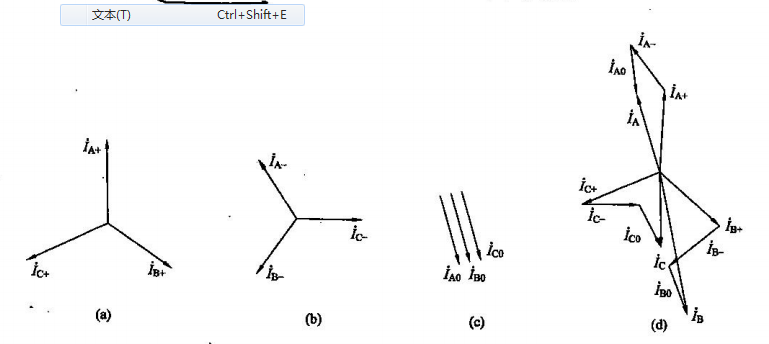
\includegraphics[width=0.80\textwidth]{4-17.png}
	\caption{对称分量法
		(a)正序电流;(b)负序电流;(c)零序电流;(d)叠加电流}
	\label{fig_4.17}
\end{figure}
所谓负序电流,是指三相电流的有效值相等、相位互差120°,相序为C→B→A,其相量关系如图\ref{fig_4.17}(b) 所示。

所谓零序电流,是指三相电流有效值相等、相位相同,其相量关系如图\ref{fig_4.17}(c)所示。

如把上述三组相序不同的对称电流,按相分别相加,即
\begin{align}
& {{{\dot{I}}}_{\text{A}}}={{{\dot{I}}}_{\text{A+}}}+{{{\dot{I}}}_{\text{A-}}}+{{{\dot{I}}}_{\text{A0}}} \\ 
& {{{\dot{I}}}_{\text{B}}}={{{\dot{I}}}_{\text{B+}}}+{{{\dot{I}}}_{\text{B-}}}+{{{\dot{I}}}_{\text{B0}}} \\ 
& {{{\dot{I}}}_{\text{C}}}={{{\dot{I}}}_{\text{C+}}}+{{{\dot{I}}}_{\text{C-}}}+{{{\dot{I}}}_{\text{C0}}}
\label{4-12}
\end{align}

由图\ref{fig_4.17}(d)可见,叠加出的${{\dot{I}}_{\text{A}}}$,${{\dot{I}}_{\text{B}}}$和${{\dot{I}}_{\text{C}}}$为一组不对称的三相电流。倒过来看,一组不对称的三相电流也一定可分解为上述三组对称分量,为了便于分解,引人复数算子$a=1/120{}^\circ $。显然, 。

对于正序电流有


\begin{align}
& {{{\dot{I}}}_{\text{B+}}}={{a}^{2}}{{{\dot{I}}}_{\text{A+}}} \\ 
& {{{\dot{I}}}_{\text{C+}}}=a{{{\dot{I}}}_{\text{A+}}} 
\label{4-13}
\end{align}

对于负序电流有
\begin{align}
& {{{\dot{I}}}_{\text{B-}}}=a{{{\dot{I}}}_{\text{A-}}} \\ 
& {{{\dot{I}}}_{\text{C-}}}={{a}^{2}}{{{\dot{I}}}_{\text{A-}}}
\label{4-14}
\end{align}

对于零序电流有
\begin{equation}
{{\dot{I}}_{\text{A0}}}={{\dot{I}}_{\text{B0}}}={{\dot{I}}_{\text{C0}}}
\label{4-15}
\end{equation}

将上面三式的关系代人式(\ref{4-12}),则得
\begin{align}
& {{{\dot{I}}}_{\text{A}}}={{{\dot{I}}}_{\text{A+}}}+{{{\dot{I}}}_{\text{A-}}}+{{{\dot{I}}}_{\text{A0}}} \\ 
& {{{\dot{I}}}_{\text{B}}}={{a}^{2}}{{{\dot{I}}}_{\text{A+}}}+a{{{\dot{I}}}_{\text{A-}}}+{{{\dot{I}}}_{\text{A0}}} \\ 
& {{{\dot{I}}}_{\text{C}}}=a{{{\dot{I}}}_{\text{A+}}}+{{a}^{2}}{{{\dot{I}}}_{\text{A-}}}+{{{\dot{I}}}_{\text{A0}}}
\label{4-16}
\end{align}

由于$1+a+{{a}^{2}}=0$,可以由式(\ref{4-16})得出
\begin{align}
& {{{\dot{I}}}_{\text{A+}}}=\frac{1}{3}\left( {{{\dot{I}}}_{\text{A}}}+a{{{\dot{I}}}_{\text{B}}}+{{a}^{2}}{{{\dot{I}}}_{\text{C}}} \right) \\ 
& {{{\dot{I}}}_{\text{A-}}}=\frac{1}{3}\left( {{{\dot{I}}}_{\text{A}}}+{{a}^{2}}{{{\dot{I}}}_{\text{B}}}+a{{{\dot{I}}}_{\text{C}}} \right) \\ 
& {{{\dot{I}}}_{\text{A0}}}=\frac{1}{3}\left( {{{\dot{I}}}_{\text{A}}}+{{{\dot{I}}}_{\text{B}}}+{{{\dot{I}}}_{\text{C}}} \right)
\label{4-17}
\end{align}
按式(\ref{4-17})求出${{\dot{I}}_{A}}$ 的三个分量后,再应用式(\ref{4-13})式(\ref{4-15}),就可求出${{\dot{I}}_{B}}$ 和${{\dot{I}}_{C}}$ 的三个分量。
应用对称分量法分析三相变压器的不对称运行,就是先把不对称电量都用三组对称的电量代替,使不对称的三相系统变换为三相对称的系统,然后对每组对称系统取一相求解,最后把计算结果叠加起来,得出三相不对称的电量数值。

\subsection{相序等效电路及其参数}
单看正序系统就是三相变压器对称运行状态,所以正序的等效电路和电路中的参数都 与对称运行时相同。

在负序系统中,三相电流和三相磁通仍是互差120°,只是超前、滞后关系与正序相反,相当于将变压器于电源的三根连线任意对调两根。单取一相分析,其内部电磁过程与正序系统完全相同。因此负序的等效电路和参数,也与对称运行时相同。

在零序系统中,三相电流和三相磁通都是同相位,它们的流通情况将受到绕组连接方式和磁路结构形式的制约。因而零序的等效电路和电路参数,在某些条件下将有别于对称运行时的情况。

1.零序励磁阻抗${{Z}_{m0}}$ 

对于零序系统,一、二次侧的漏阻抗与正、负序系统相同,这是因为:①每相绕组的电阻不受电流相位关系的影响;②各相绕组的漏磁通分别有自己的流通空间,所以每相的漏感抗也不随三相电流相位关系的改变而改变。励磁阻抗是代表主磁通在电路中的作用的参数,而零序主磁通的流通情况与磁路结构形式有关,不同的磁路结构将有不同的零序励磁阻抗值。

(1)三相变压器组的三相磁路分别独立,三相同相位的零序磁通互不影响地流过各自的磁路,它所受到的磁阻与正序、负序时相同,因而三相变压器组的零序励磁阻抗与对称运行时相同,即${{Z}_{m0}}={{Z}_{m}}$。

(2)三相心式变压器的三相磁路互为回路,而三相同相位的零序磁通在任何瞬间都大小相等、流通方向相同,因而无法在铁心中闭合,只能分别穿过变压器油经邮箱壁流通。这时磁通所遇到的磁阻很大,一定的励磁电流所产生的磁通和感应电动势将比对称运行时小的多,所以零序励磁阻抗的数值将远小于对称运行时的励磁阻抗,即$\left| {{Z}_{m0}} \right|\ll \left| {{Z}_{m}} \right|$。

2.零序等效电路

由于三相零序电流有效值相等、相位相同,所以绕组的连接方式直接影响着它的流通情况。当绕组接成星形无中性线时,零序电流无法流通,其等效电路应画成断路。当绕组接成星形有中性线时,三相同相位的零序电流都通过中性线流回[见图\ref{fig_4.18}(a)],中线中电流为${{\dot{I}}_{A0}}+{{\dot{I}}_{B0}}+{{\dot{I}}_{C0}}=3{{\dot{I}}_{A0}}$。可见,每相的零序电流都可顺利地通过绕组和端线,因此,其等效电路与对称运行时完全相同。

当绕组接成三角形时,三相中的零序电流构成一闭合环流,而在端线中无零序电流[见图\ref{fig_4.18}(b)]。

因此,这时的等效电路应是在绕组内部为通路,绕组对外(一次侧对电源,二次侧对负载)为断路。

下面以常见的Yyn和YNd两种连接组为例,介绍零序等效电路的画法。

(1)	Yyn连接组。这种连接的零序电流是由于二次侧负载阻抗不对称或电压不对称使中性线中有电流引起的。一次侧无零序电流,仅有零序感应电动势,其等效电路如图\ref{fig:4.19}所示。

(2)	YNd连接组。这种连接的零序电流是由于电源中有零序电压引起的。一、二次侧都能流过零序电流,但在二次侧不能流向负载电路,其等效电路如图\ref{fig:4.20}所示。

\begin{figure}[H]
	\centering
	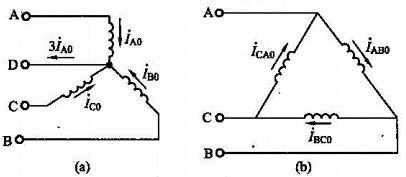
\includegraphics[width=0.80\textwidth]{4-18.png}
	\caption{零序电流的流通情况
		(a)星形结构;(b)三角形结构}
	\label{fig_4.18}
\end{figure}
\begin{figure}  
	\begin{minipage}[H]{0.45\linewidth}  
		\centering  
		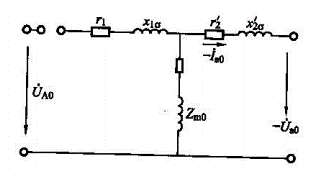
\includegraphics[width=2.2in]{4-19.png}  
		\caption{Yyn的零序等效电路}  
		\label{fig:4.19}  
	\end{minipage}
	\begin{minipage}[H]{0.45\linewidth}  
		\centering  
		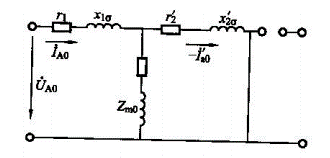
\includegraphics[width=2.2in]{4-20.png}  
		\caption{YNd的零序等效电路}  
		\label{fig:4.20}  
	\end{minipage}  
\end{figure}

\subsection{Yyn0连接组的单相负载运行}

现在以Yyn0连接组单相负载运行为例,介绍用对称分量法分析三相变压器不对称运行的过程。其电路如图\ref{fig_4.21}所示,此时有
\begin{align}
& {{{\dot{I}}}_{a}}=\dot{I} \\ 
& {{{\dot{I}}}_{b}}={{{\dot{I}}}_{c}}=0 \\ 
& {{{\dot{U}}}_{a}}={{{\dot{I}}}_{a}}{{Z}_{L}}
\label{4-18}
\end{align}

\begin{figure}[H]
	\centering
	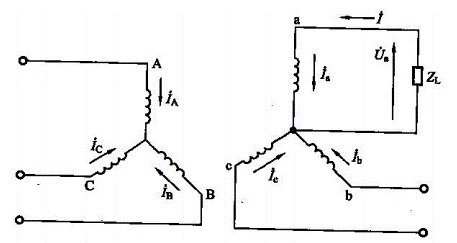
\includegraphics[width=0.80\textwidth]{4-21.png}
	\caption{Yyn0单相负载电路}
	\label{fig_4.21}
\end{figure}

\subsubsection{求二次侧单相负载电流$\dot{I}$}
应用对称分量法求二次侧电流的各序分量为
\begin{align}
& {{{\dot{I}}}_{\text{a+}}}=\frac{1}{3}\left( {{{\dot{I}}}_{\text{a}}}+a{{{\dot{I}}}_{\text{b}}}+{{a}^{2}}{{{\dot{I}}}_{\text{c}}} \right)=\frac{1}{3}{{{\dot{I}}}_{\text{a}}}=\frac{1}{3}\dot{I} \\ 
& {{{\dot{I}}}_{\text{a-}}}=\frac{1}{3}\left( {{{\dot{I}}}_{\text{a}}}+{{a}^{2}}{{{\dot{I}}}_{\text{b}}}+a{{{\dot{I}}}_{c}} \right)=\frac{1}{3}{{{\dot{I}}}_{\text{a}}}=\frac{1}{3}\dot{I} \\ 
& {{{\dot{I}}}_{\text{a0}}}=\frac{1}{3}\left( {{{\dot{I}}}_{\text{a}}}+{{{\dot{I}}}_{\text{b}}}+{{{\dot{I}}}_{\text{c}}} \right)=\frac{1}{3}{{{\dot{I}}}_{\text{a}}}=\frac{1}{3}\dot{I} 
\label{4-19}
\end{align}

为便于分析,正序和负序都采用简化等效电路。因为电源是三相对称的,所以一次侧外 加电压中只有正序分量,负序和零序电压为零。各序等效电路如图\ref{fig_4.22}所示,应用克希荷夫定律可得

\begin{align}
& {{{\dot{U}}}_{A+}}=-{{{{\dot{I}}'}}_{a+}}{{Z}_{k}}+{{{\dot{U}}}_{a+}} \\ 
& 0=-{{{{\dot{I}}'}}_{a-}}{{Z}_{k}}+{{{\dot{U}}}_{a-}} \\ 
& 0=-{{{{\dot{I}}'}}_{a0}}\left( {{Z}_{m0}}+{{{{Z}'}}_{2}} \right)+{{{\dot{U}}}_{a0}} 
\label{4-20}
\end{align} 

\begin{figure}[H]
	\centering
	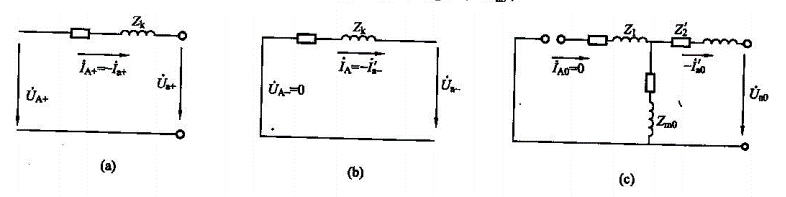
\includegraphics[width=0.80\textwidth]{4-22.png}
	\caption{Yyn0的各序等效电路
		(a)正序(b)负序(c)零序}
	\label{fig_4.22}
\end{figure}

将式(\ref{4-20})中三等式相加,并考虑到
\begin{equation}
{{\dot{I}}_{a+}}={{\dot{I}}_{a-}}={{\dot{I}}_{a0}}=\frac{1}{3}\dot{I}
\label{4-21}
\end{equation}

\begin{equation}
{{\dot{U}}_{a+}}+{{\dot{U}}_{a-}}+{{\dot{U}}_{a0}}={{\dot{U}}_{a}}={{\dot{I}}_{a}}{{Z}_{L}}=\dot{I}{{Z}_{L}}
\label{4-22}
\end{equation}

可得	
\begin{equation}
{{\dot{U}}_{A+}}=-\frac{1}{3}{\dot{I}}'\left( 2{{Z}_{k}}+{{{{Z}'}}_{2}}+{{Z}_{m0}} \right)+\left( -{\dot{I}}'{{{{Z}'}}_{L}} \right)
\label{4-23}
\end{equation}

所以单相负载电流的归算值为

\begin{equation}
-{\dot{I}}'=\frac{{{{\dot{U}}}_{A+}}}{\frac{2}{3}{{Z}_{k}}+\frac{1}{3}{{{{Z}'}}_{2}}+\frac{1}{3}{{Z}_{m0}}+{{{{Z}'}}_{L}}}
\label{4-24}
\end{equation}

\subsubsection{求一次侧各相电流}
忽略励磁电流,根据磁动势平衡可由二次侧${{\dot{I}}_{a}}$的各序分量求得一次侧${{\dot{I}}_{A}}$ 的对应分量。不过由于一次侧没有中性线,零序电流无法流通,所以${{\dot{I}}_{A}}$ 的三个对称分量为
\begin{align}
& {{{\dot{I}}}_{A+}}=-{{{{\dot{I}}'}}_{a+}}=-\frac{1}{3}{\dot{I}}' \\ 
& {{{\dot{I}}}_{A-}}=-{{{{\dot{I}}'}}_{a-}}=-\frac{1}{3}{\dot{I}}' \\ 
& {{{\dot{I}}}_{A0}}=0
\label{4-25}
\end{align}	
一次侧各相电流分别为
\begin{align}
& {{{\dot{I}}}_{A}}={{{\dot{I}}}_{A+}}+{{{\dot{I}}}_{A-}}+{{{\dot{I}}}_{A0}}=-\frac{2}{3}{\dot{I}}' \\ 
& {{{\dot{I}}}_{B}}={{a}^{2}}{{{\dot{I}}}_{A+}}+a{{{\dot{I}}}_{A-}}+{{{\dot{I}}}_{A0}}=\frac{1}{3}{\dot{I}}' \\ 
& {{{\dot{I}}}_{C}}=a{{{\dot{I}}}_{A+}}+{{a}^{2}}{{{\dot{I}}}_{A-}}+{{{\dot{I}}}_{A0}}=\frac{1}{3}{\dot{I}}'
\label{4-26}
\end{align}	
可见,单相负载时,二次侧只有a相有电流$\dot{I}$,一次侧A相电流一半经B相,另一半经C相流回电源。

\subsubsection{Yyn连接的三相变压器组不能带单相负载}

现在对单相负载电流$I$的大小作进一步的分析。在式(\ref{4-24})的分母中,${{Z}_{k}}$ 和${{Z}_{2}}$远小于${{Z}_{m0}}$和${{{Z}'}_{L}}$,如把它们略去,则得
\begin{equation}
-\dot{I}=\frac{{{{\dot{U}}}_{A+}}}{\frac{1}{3}{{Z}_{m0}}+{{{{Z}'}}_{L}}}
\label{4-27}
\end{equation}

可见,$\dot{I}$的大小不仅取决于负载阻抗${{Z}_{L}}$,还要受零序励磁阻抗${{Z}_{m0}}$的影响。

对于三相变压器组,其${{Z}_{m0}}$ 等于对称运行时的励磁阻抗${{Z}_{m}}$,其值比${{{Z}'}_{L}}$大得多,因而$\dot{{I}'}$ 的值很小。也就是说,无论怎样减小负载阻抗${{Z}_{L}}$,通过负载的电流$I$ 也大不起来。取极端情况,令${{Z}_{L}}=0$,$\dot{{I}'}$为单相短路电流,其值为
\begin{equation}
-\dot{{I}'}=\frac{3{{{\dot{U}}}_{A+}}}{{{Z}_{m0}}}=3{{\dot{I}}_{0}}
\label{4-28}
\end{equation}
只有空载电流的3倍,而变压器的空载电流是很小的。

通过上面的分析,可以得出结论,即Yyn连接的三相变压器组不能带单相负载。

而对于三相心式变压器,其${{Z}_{m0}}$值不大,单相电流${I}'$的大小主要取决于负载阻抗${{{Z}'}_{L}}$,所以Yyn连接的三相心式变压器可以带单相负载运行。

\subsubsection{“中性点移动”现象}

根据式(\ref{4-18}),单相负载电流$\dot{I}=\frac{{{{\dot{U}}}_{a}}}{{{Z}_{L}}}$。对于三相变压器组,随着${{Z}_{L}}$ 的减小,$I$增加很少,这说明${{U}_{a}}$ 不是恒量,随着$I$的增大${{U}_{a}}$必将显著变小。引起这种现象的主要原因是由于零序磁通在一、二次绕组中产生了三相同相位的零序电动势。现进行如下分析。

(1)在正序系统中,一、二次侧正序电流通过磁动势平衡产生一定的正序磁通,其大小取决于一次侧外加电压(${{\Phi }_{m}}\approx \frac{{{U}_{1}}}{4.44f{{W}_{1}}}$)。正序磁通在一次侧产生三相正序电动势以平衡对称的外加电压;在二次侧产生三相对称电动势${{\dot{E}}_{a+}}$ 、${{\dot{E}}_{b+}}$ 、${{\dot{E}}_{c+}}$,其相量在图\ref{fig_4.23}中分别用矢量oa、ob和oc表示。
\begin{figure}[H]
	\centering
	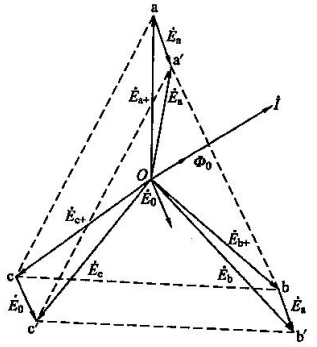
\includegraphics[width=0.80\textwidth]{4-23.png}
	\caption{中点移动}
	\label{fig_4.23}
\end{figure}

(2)在负序系统中,由于外加电压中无负序分量,所以一次侧不要求有负序磁通来产生负序电动势。当二次侧的负序电流产生负序磁动势时,一次侧的负序电流将立即产生一个抵消它的磁动势,从而使铁心中的负序磁通接近于零。由负序磁通在一、二次侧所产生的负序电动势也基本为零。

(3)在零序系统中,因为外加电压中无零序分量,按一次侧电压平衡要求,也希望零序磁通为零。但是由于一次侧无零序电流,无法抵消由二次侧零序电流所产生的磁动势,于是在铁心中就产生了一定大小的零序磁通。它在一、二次侧产生三相同相位的零序电动势${{\dot{E}}_{0}}$ 叠加在正序电动势上就形成了三相不对称的电动势。二次侧三相电动势的相量在图\ref{fig_4.23}中分别为矢量oa',ob'和oc'。

在图\ref{fig_4.23}中,零序电动势${{\dot{E}}_{0}}$滞后于零序磁通${{\dot{\Phi }}_{0}}90{}^\circ $,而${{\dot{\Phi }}_{0}}$与${{\dot{I}}_{0}}=\frac{1}{3}\dot{I}$ 同相位,${{\dot{I}}_{0}}$与${{\dot{E}}_{a}}$的相位差则主要取决于单相负载的性质(即${{Z}_{L}}$的抗阻比)。没有零序磁动势${{\dot{E}}_{0}}$时,中点O处在$\Delta abc$的中心;有了${{\dot{E}}_{0}}$后,三相电动势三角形为$\Delta {a}'{b}'{c}'$,这时O点已不在三角 形的中心。这就是所谓的"中性点移动"现象,其实质就是带单相负载的相电压降低,另外两相电压升高。这种现象不只是在单相负载时发生,只要三相不对称,并在二次侧出现零序电流${{I}_{0}}$,就将产生零序磁通${{\Phi}_{0}}$和零序电动势${{E}_{0}}$。比如当a相负载很多,b、c相负载很少时,也会产生较大的${{I}_{0}}$、${{\Phi }_{0}}$也和${{E}_{0}}$,结果使a 相电压降低,b、c相电压升高,这就影响到用电设备的正常工作,严重时可能造成用电设备的损坏。因此,三相变压器组不采用Yyn0连接组。

对于三相心式变压器,零序磁通所遇到的磁阻很大,${{\Phi }_{0}}$和${{E}_{0}}$都较小,再加上使用中要限制三相不对称的程度,所以其“中性点移动”现象不明显。

\end{document}